%!TEX root = ../thesis.tex
\graphicspath{ {Figs/Chapter2/} }

\section {Introducción y conceptos blockchain}  %Title of the First Chapter

\subsection{Blockchain}
%\textcolor{red}{Creo que ésta debería ser la primera sección de este capítulo. Dar una explicación general de lo qué es blockchain (al estilo de https://en.wikipedia.org/wiki/Blockchain), que es una cadena de bloques que crece, lo que contiene cada bloque, que los nuevos bloques se validadn en en red p2p a través de mecanismos de consenso, el asunto distribuido y tolerante  faalas, incluso agregar dibujos para que sea más claro. Es decir dar los términos claves en un párrafo y luego ir con más detalle como lo que ya tienes aquí.}


El  \textit{blockchain}, también conocido como libro de contabilidad distribuido, es una base de datos descentralizada y distribuida que registra bloques de información y los entrelaza para facilitar la recuperación de la información y la verificación de que ésta no ha sido cambiada mediante técnicas criptográficas. Los bloques de información se enlazan mediante apuntadores {\it hash}(estructura de datos que asocia llaves o claves con valores) que conectan el bloque actual con el anterior y así sucesivamente hasta llegar al bloque inicial o \textbf{bloque génesis}. La Figura \ref{blockchain_linkedlist} muestra gráficamente el concepto de \textit{blockchain}.
El \textit{blockchain} es almacenado por todos aquellos nodos de la red que siguiendo un protocolo apropiado para las operaciones efectuadas sobre la plataforma, logran alcanzar un consenso sobre la integridad de sus datos~\cite{staff2016blockchains}~\cite{neittaanmaki2016blockchain}.

\begin{figure}[H]
    \centering
    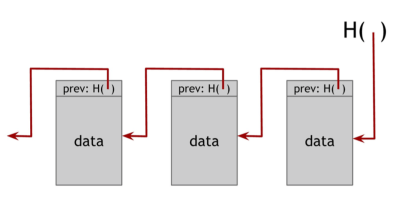
\includegraphics[width=0.8\textwidth]{cadena_de_bloques.png}
     \caption{\textit{Blockchain}: lista enlazada de bloques construida con apuntadores hash. Fuente: \textit{Bitcoin and Cryptocurrency Technologies Book. Princeton University}.\cite{narayanan2016bitcoin}}
    \label{blockchain_linkedlist}
\end{figure}


Desde el punto de vista de negocios, el \textit{blockchain} se  define como una plataforma de tipo \textit{P2P} (por sus siglas en inglés Peer-to-Peer),  mediante la cual los pares pueden intercambiar valores usando transacciones sin la necesidad de un árbitro central de confianza. Esto permite que \textit{blockchain} sea un mecanismo de consenso descentralizado donde ninguna autoridad única está a cargo de la base de datos~\cite{bashir2017mastering}.

Dadas las características y propiedades antes expuestas, la tecnología \textit{blockchain}  se adapta especialmente a escenarios en los que se requiera almacenamiento cronológico de datos, inmutables y cuya confianza no prevalezca en un ente central de control, sino en los participantes involucrados~\cite{wiki:CadenaBloques}.

Dentro de los elementos generales que debería contener cualquier plataforma \textit{blockchain} se encuentran:
\begin{itemize}
    \item Direcciones: las direcciones son identificadores únicos que se utilizan en una transacción dentro del \textit{blockchain} para designar remitentes y destinatarios. Una dirección generalmente es una clave pública. Si bien las direcciones pueden ser reutilizadas por el mismo usuario, las direcciones son únicas. En la práctica, sin embargo, un solo usuario no puede usar la misma dirección nuevamente y generar una nueva para cada transacción. 
    \item Transacción: Una transacción es la unidad fundamental del \textit{blockchain}. Una transacción representa una transferencia de valor de una dirección a otra.
    \item Bloque: Un bloque se compone de varias transacciones y otros elementos como el {\it hash} del bloque anterior ({\it hash pointer}), {\it marca de tiempo} y {\it banderas(bits predefinidos que contienen valores binarios)}.
    \item Red punto-a-punto (P2P): ésta es una topología de red mediante la cual todos los compañeros (nodos de la red) se pueden comunicar entre sí y enviar y recibir mensajes.
    \item {\it Scripting} o lenguaje de programación: los {\it scripts} de transacción son conjuntos de comandos predefinidos para que los nodos transfieran tokens de una dirección a otra y realicen otras funciones. Una característica deseable de los lenguajes utilizados dentro del \textit{blockchain} es que sean “Turing completos”.
    \item Contratos Inteligentes: programas que se ejecutan sobre el \textit{blockchain} y encapsulan la lógica de negocios que se ejecutará cuando se cumplan ciertas condiciones. La función de contrato inteligente no está disponible en todas las cadenas de bloques, pero ahora se está convirtiendo en una característica muy deseable debido a la flexibilidad y la potencia que proporciona a las aplicaciones \textit{blockchain}.
    \item Máquina Virtual: Una máquina virtual permite que el código Turing completo se ejecute en el \textit{blockchain} (como contratos inteligentes), a diferencia  de un {\it script} de transacción que puede estar limitado en su funcionamiento. Las máquinas virtuales no están disponibles en todas las plataformas  \textit{blockchains}; sin embargo, varios plataformas actuales usan máquinas virtuales para ejecutar programas, por ejemplo, Ethereum Virtual Machine (EVM) y Chain Virtual Machine (CVM).
    \item Nodos: Un nodo en una red \textit{blockchain} realiza varias funciones dependiendo del rol que desempeña. Un nodo puede proponer y validar transacciones y realizar operaciones de minería para facilitar el consenso y asegurar la plataforma \textit{blockchain}. Esto se hace siguiendo un protocolo o algoritmos de consenso explicados a continuación. Los nodos también pueden realizar otras funciones, como la verificación simple de pagos (nodos livianos), validadores y muchas otras funciones según el tipo de \textit{blockchain} utilizada y el rol asignado al nodo.
\end{itemize}

\textbf{Características principales}
\begin{itemize}
    \item Consenso Distribuido: El consenso distribuido es el principal soporte de una plataforma \textit{blockchain}. Esto permite que el \textit{blockchain} presente una única versión de la verdad acordada por todas las partes sin el requisito de una autoridad central.
    \item Verificación de transacciones: Todas las transacciones publicadas por los  nodos en el \textit{blockchain} se verifican en base a un conjunto predeterminado de reglas y sólo se seleccionan las transacciones válidas para su inclusión en un bloque.
    \item Transferencia de valores entre pares: El \textit{blockchain} permite la transferencia de valor entre sus usuarios a través de tokens(unidad de valor que una organización crea para gobernar su modelo de negocio). Se puede pensar que los tokens son portadores de valor.
    \item Generación de criptomonedas: En un \textit{blockchain} se  puede generar criptomonedas como un incentivo para sus mineros que validan las transacciones y gastan recursos para asegurar la plataforma. Esta es una función opcional según el tipo de \textit{blockchain} utilizado.
    \item Propiedad intelectual: Es posible vincular un elemento digital o físico al \textit{blockchain} de una manera irrevocable, de modo que no pueda ser reclamado por nadie más; el propietario tiene el control total de su activo y no puede ser gastado doblemente o tener doble propiedad. Esta característica tiene implicaciones de gran alcance, especialmente en la gestión de derechos digitales y en los sistemas electrónicos de efectivo, donde la detección de doble gasto es un requisito clave
    \item Proveedor de seguridad: El \textit{blockchain} se basa en una tecnología criptográfica comprobada que garantiza la integridad y la disponibilidad de los datos. Generalmente, la confidencialidad no se proporciona en primera instancia debido a los requisitos de transparencia(transacciones publicas y visibles para cualquier usuario asociado o no la red blockchain), sin embargo la investigación en esta área ha  madurado y se ha avanzado mucho para obtener confidencialidad y privacidad en las plataformas \textit{blockchain} que necesiten de estas características.
    \item Inmutabilidad: Otra característica clave de \textit{blockchain} es el hecho que los registros que se agregan una vez a la plataforma son inmutables. Aunque teóricamente existe la posibilidad de revertir los cambios, en la práctica se considera casi imposible de lograr, ya que se requiere de una cantidad inaccesible de recursos informáticos, ya que se tendría que accesar a cada uno de los nodos que comparten el registro, alterar cada una de sus decisiones y todo esto en simultaneo, necesitando gran poder de computo para cumplir dicho objetivo.
    \item Unicidad: Esta característica del \textit{blockchain} garantiza que cada transacción sea única y no se haya consumido anteriormente. Esto es especialmente relevante en las plataformas \textit{blockchain} de criptomonedas donde la detección y  evasión  del “doble gasto” son un requisito clave.
\end{itemize}

La Figura~\ref{blockchain_properties} muestra las características de la tecnología \textit{blockchain}.

\begin{figure}[h]
    \centering
    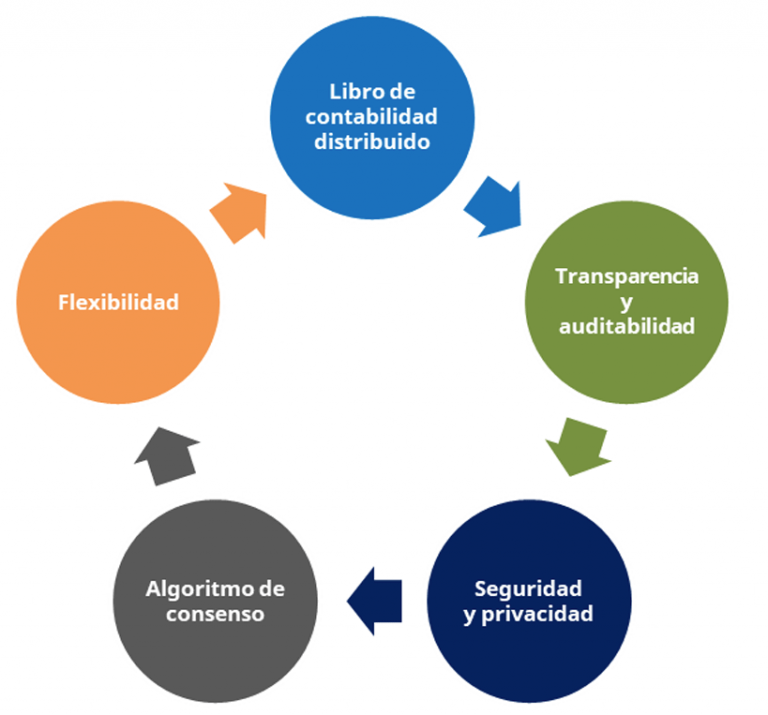
\includegraphics[width=0.5\textwidth]{caracteristicas_blockchain.png}
     \caption{Caracertisticas principales de la tecnologia \textit{blockchain} }
    \label{blockchain_properties}
\end{figure}



\textbf{Tipos de plataformas \textit{blockchain}}:  Basado en la evolución del \textit{blockchain} en los últimos años, esta tecnología se puede dividir en varios tipos con atributos distintos que en muchos casos suelen solaparse:

\begin{itemize}
    \item Públicos:  Estos  tipos de \textit{blockchain}s están abiertos al público y cualquiera puede participar como un nodo en el proceso de toma de decisiones y éstos  pueden o no ser recompensados por su participación. Los registros son propiedad de nadie y están públicamente abiertos para que cualquier persona participe y consulte. Todos los usuarios  mantienen una copia del \textit{blockchain} en sus nodos locales y utilizan un mecanismo de consenso distribuido para tomar una decisión sobre el eventual estado del mismo. Este tipo  también se conocen como libros no permisados.
    \item Privadas: Como su nombre lo indica son privadas y están abiertas sólo a un consorcio o grupo de individuos u organizaciones que han decidido compartir el libro de contabilidad entre ellos.
    \item Semi-privadas: En este tipo de plataformas \textit{blockchain}, una parte del mismo es privada y la otra es pública. La parte privada está controlada por un grupo de individuos, mientras que la parte pública está abierta para la participación de cualquier persona.
    \item Libros contable autorizado: Un libro de contabilidad autorizado es un \textit{blockchain} por el cual los participantes de la red son conocidos y de confianza. Los libros mayores autorizados no necesitan usar un mecanismo de consenso distribuido, en su lugar se puede usar un protocolo de acuerdo para mantener una versión compartida de la verdad sobre el estado de los registros en el \textit{blockchain}. Tampoco es obligatorio que una plataforma \textit{blockchain} autorizada sea privada, ya que puede ser un \textit{blockchain} público, pero con control de acceso regulado.
    \item Libros contable distribuido: Este libro se distribuye entre sus participantes y se extiende a través de múltiples sitios u organizaciones. Este tipo puede ser privado o público. La idea clave es que, a diferencia de muchas otras plataformas \textit{blockchain}, los registros se almacenan de forma contigua en lugar de ordenarse en bloques.
    \item Tokenisadas: Son \textit{blockchain}s estándar que generan criptomonedas como resultado de un proceso de consenso a través de la minería o mediante la distribución inicial. Aquí entra cualquier plataforma relacionada a criptomonedas.
\end{itemize}

\subsection {Sistemas distribuidos}

Primeramente es necesaria la  comprensión de los sistemas distribuidos porque  la tecnología de \textit{blockchain} en su núcleo es un sistema distribuido, específicamente, un sistema distribuido descentralizado.

Los sistemas distribuidos son un paradigma informático mediante el cual dos o más nodos trabajan entre sí en una manera coordinada para lograr un resultado común y está modelada de tal manera que los usuarios finales lo ven como una única plataforma lógica~\cite{bashir2017mastering}.

Se define un nodo como un jugador individual en un sistema distribuido. Todos los nodos son capaces de enviar y recibir mensajes hacia y desde un nodo a otro. Cada nodo posee memoria y procesador propios y se clasifican en tres tipos:  honestos, defectuosos y maliciosos.
%, poseen  memoria y procesador propios. 
Un nodo que puede mostrar un comportamiento arbitrario también se conoce como nodo bizantino. Este comportamiento arbitrario puede ser intencionalmente malicioso, lo cual es perjudicial para el funcionamiento de la red. En general, cualquier comportamiento inesperado de un nodo en la red se puede categorizar como nodo bizantino.

El principal desafío que se presenta en los sistemas distribuidos es la coordinación entre nodos y tolerancia a fallas. Si algunos de los nodos se vuelven defectuosos o se rompen enlaces de red, el sistema distribuido debería ser capaz de  tolerar este tipo de situación y mantener su funcionamiento sin problemas para lograr el resultado deseado.


\subsection{Consenso}
El consenso es un proceso de acuerdo entre nodos desconfiados sobre un estado final de datos. Para lograr el consenso, se pueden usar diferentes algoritmos. En general es fácil llegar a un acuerdo entre dos nodos (por ejemplo en esquemas cliente-servidor) pero cuando múltiples nodos participan en un sistema distribuido y necesitan ponerse de acuerdo en un solo valor, se vuelve complejo lograr dicho consenso. El concepto que define la obtención de consenso entre nodos múltiples se conoce como consenso distribuido (ver Figura~\ref{blockchain_consensus})~\cite{bashir2017mastering}. 

\begin{figure}[h]
    \centering
    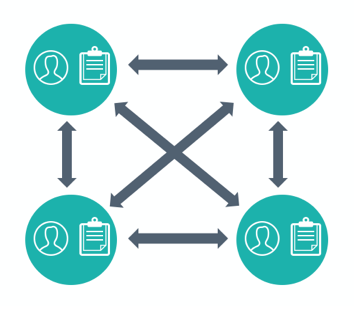
\includegraphics[width=0.4\textwidth]{consenso-nodos.png}
     \caption{Ejemplo de nodos efectuando consenso}
    \label{blockchain_consensus}
\end{figure}

\textbf{Mecanismos de consenso:}  Un mecanismo de consenso es un conjunto de pasos que toman todos, o la mayoría de los nodos, para acordar un estado o valor propuesto~\cite{swanson2015consensus}. Los mecanismos de consenso han pasado recientemente a ser el centro de atención y ganó mucha popularidad con el advenimiento de la primera implementación pública de \textit{blockchain}, la famosa plataforma Bitcoin \cite{nakamoto2008bitcoin}.

Existen cinco requisitos que deben cumplirse para proporcionar los resultados deseados en un mecanismo de consenso:

\begin{itemize}
\item Acuerdo: todos los nodos confiables deciden sobre el mismo valor.
\item Terminación: todos los nodos confiables terminan la ejecución del proceso de consenso y eventualmente llegan a una decisión.
\item Validez: el valor acordado por todos los nodos honestos debe ser el mismo que el valor inicial propuesto por al menos un nodo confiable.
\item Tolerante a fallas: el algoritmo de consenso debería poder ejecutarse en presencia de fallas o nodos maliciosos (nodos bizantinos).
\item Integridad: este es un requisito donde ningún nodo toma la decisión más de una vez. Los nodos toman decisiones solo una vez en un solo ciclo de consenso.
\end{itemize}

Existen varios tipos de mecanismo de consenso, dentro de los dos mas comunes encontramos:
%, dentro de los 2 mas comunes encontramos:
\begin{itemize}
\item Basados en la tolerancia a fallas bizantinas: sin operaciones de cálculo intensivo, como la inversión de hash parcial, este método se basa en un esquema simple de nodos que publican mensajes firmados. Eventualmente, cuando se recibe una cierta cantidad de mensajes, se llega a un acuerdo. Una de las implementaciones más famosas de este tipo, es  el  algoritmo Paxos publicado por Leslie Lamport~\cite{lamport2001paxos}.

\item Basados en líderes: este tipo de mecanismo requiere que los nodos compitan por la lotería de elección de líderes y el nodo que los gana proponga un valor final. Dentro de las implementaciones conocidas de este tipo, destaca el protocolo RAFT publicado por Diego Ongaro y John Ousterhout~\cite{ongaro2015raft}.
\end{itemize}

El concepto de consenso de sistemas distribuidos ha sido incorporado  en la tecnología \textit{blockchain} para proporcionar un medio de aceptación y validación única de la verdad por parte de todos los pares en la red \textit{blockchain}. Dentro de los \textbf{algoritmos de consenso} más importantes que están disponibles hoy o están siendo investigados en el contexto de \textit{blockchain} sobresalen:

\begin{itemize}
\item Prueba de trabajo: este tipo de mecanismo de consenso se basa en la prueba del consumo de recursos computacionales suficientes  antes de proponer un valor para su aceptación por parte de la red. Este mecanismo es utilizado en la plataforma Bitcoin  y otras plataformas \textit{blockchain} asociadas a criptomonedas.
\item Prueba de apuesta: este algoritmo funciona con la idea de que un nodo o usuario tiene una apuesta suficiente en el sistema; por ejemplo, el nodo ha invertido los recursos suficientes  para que cualquier intento de  perjudicar o comprometer a la red concluiria en una perdida de sus propios recursos invertidos. Esta idea fue presentada por el proyecto de Peercoin y se encuentra en etapa de prueba  en el \textit{blockchain} de Ethereum. Otro concepto importante en este tipo de algoritmo es la “edad de la moneda”, que es un derivado desde la cantidad de tiempo y la cantidad de monedas que no se han gastado. En este modelo, las posibilidades de proponer y firmar el siguiente bloque aumentan con la edad de la moneda.
\item Prueba de importancia: esta prueba comparte similitud con la “Prueba de Apuesta” sin embargo este mecanismo no solo se basa en la cantidad de  apuesta que tiene un usuario en el sistema, sino que adicionalmente monitorea el uso y movimiento de los tokens por parte del usuario para establecer un nivel de confianza e importancia. Este mecanismo es utilizado en el proyecto Nemcoin.
\item Prueba de tiempo transcurrido: introducido por Intel, usa un Entorno Confiable de Ejecución (TEE por sus siglas en inglés) para proporcionar aleatoriedad y seguridad en el proceso de elección del líder a través de un tiempo de espera garantizado. Requiere el Intel SGX (Software Guard Extension) procesador para proporcionar la garantía de seguridad\cite{costan2016intel}.
\item Consenso federado o consenso bizantino federado: los nodos en este protocolo mantienen un grupo de pares y compañeros de confianza pública y propaga sólo aquellas transacciones que han sido validadas por la mayoría de los nodos de confianza. Usados en el protocolo de consenso del proyecto Stellar\cite{stellarProject:stellarBasics}
\item Mecanismos basados  en reputación: mecanismo donde un líder es elegido sobre la base de la reputación que ha construido con el tiempo en la red. Esto puede basarse en la votación de otros miembros.
\end{itemize}

